\section{Related Work}

\subsection{Imitation Learning under Partial Observability}
Standard imitation learning assumes Markovian observations, causing reactive visuomotor policies to fail under partial observability. Belief-state space methods address this issue by explicitly modeling task state but require task-specific representations and update rules~\cite{aastrom1965optimal}.
Recent work instead incorporates explicit memory into policy. Some methods rely on object-centric representations to reduce the amount of information, but often limit retrieval to spatial information~\cite{sam2act}. Others retrieve past observations using similarity in learned semantic embeddings, leveraging pretrained vision-language models~\cite{clipnav,okrobot}, or apply hand-designed rules for memory filtering~\cite{memer}.
Such assumptions restrict their applicability to settings where task-relevant information is well captured by a fixed representation or retrieval rule (here, a semantic one), and may not scale to more diverse long-horizon tasks.

Several approaches learn compact representations of the history to support long-horizon reasoning~\cite{fang2019scene}. While effective, learned compression can discard granular information, such as low-level action sequences taken by the robot. These limitations motivate memory retrieval mechanisms that can flexibly access diverse task-relevant information from history without relying on task-specific designs.

\subsection{Knowledge Distillation from Foundation Models}
Vision-language foundation models encode rich knowledge about scenes, objects, and activities from large-scale multimodal data and have been widely used in robotics for perception, planning, affordance learning, and semantic reasoning~\cite{shridhar2022cliport,song2023llm,ahn2022can,gu2023rt,nasiriany2025rt,shah2025bumble}.
Prior work has also distilled knowledge from foundation models into robotic systems by improving parametric representations~\cite{zhou2025chatvla,driess2025knowledge}. In contrast, relatively little work has explored using foundation models to guide memory retrieval in visuomotor imitation learning, that is, learning to retrieve information from non-parametric memory~\cite{lewis2020retrieval}. Our work builds on these efforts by distilling task-relevant priors from vision-language models to supervise learned memory retrieval, while grounding the policy through action imitation.

\begin{figure*}[t]
    \centering
    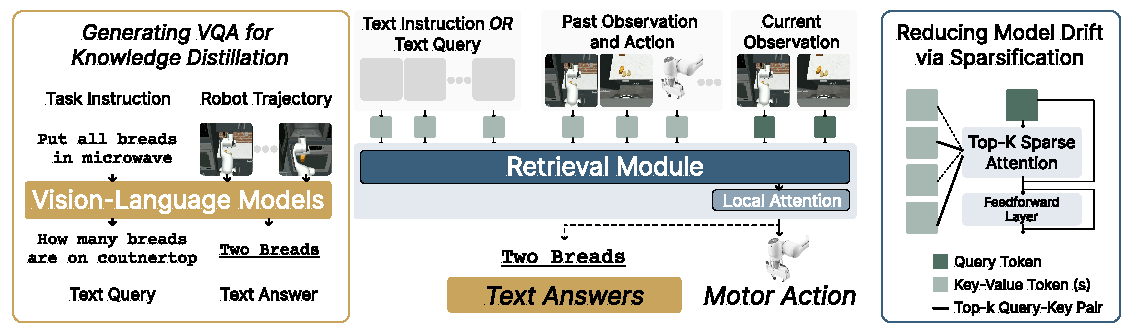
\includegraphics[width=\textwidth]{figures/method_overview_new.pdf}
    \vspace{-20pt}
    \caption{\textbf{Overview.} \ourmethod{} learns a visuomotor policy that retrieves information from the past observations and actions to predict low-level robot actions (middle), guided by priors from vision-language models to retrieve task-relevant information through VQA (left) and uses sparse attention to reduce model drift (right).}
    \label{fig:method_overview}
    \vspace{-10pt}
\end{figure*}
\subsection{Memory Mechanisms for Long-Context Reasoning}
Modeling long-range temporal dependencies is a central challenge in sequential decision making. 
Recurrent and state-space models maintain memory through compressed latent states but struggle with selective recall and credit assignment over long horizons~\cite{lstm, mamba, bengio1993credit}.
Transformer-based models address these limitations by using attention to directly access past inputs~\cite{vaswani2017attention}.
However, dense attention over long contexts can cause irrelevant or noisy information to increasingly influence predictions~\cite{hong2025context}, an issue that is especially pronounced in robotics due to prediction errors and compounding errors during closed-loop execution.

To regulate information flow in long-context models, prior work has proposed combining attention with recurrence~\cite{dai2019transformer}, a gating mechanism~\cite{gatedattention}, and inducing sparsity in the transformer architecture~\cite{zaheer2020big}.
While these mechanisms have been extensively studied in language and vision, their effectiveness in long-horizon closed-loop visuomotor control has received less attention.
In this work, we find that simple Top-$K$ attention sparsification is effective for reducing the influence of accumulated error in model prediction.
% \begin{itemize}
%     \item Recurrent and state-space sequence models (e.g., LSTM, GRU, Mamba) maintain memory in compressed latent states, which limits selective recall of past information and leads to poor credit assignment over long horizons.
%     \item Transformer-based models enable direct access to long histories through attention, avoiding recurrence-based credit assignment issues.
%     \item However, dense attention over long sequences leads to \emph{context rot}, where irrelevant or noisy past information increasingly influences decision making over time.
%     \item This problem is much more prevalent in robotics because the noise is confounded from the model prediction as well as the environment 
%     \item To address this, prior work in machine learning proposes various mechanisms to regulate information flow, including combining attention with recurrence, sink or summary tokens, hierarchical attention, bias tuning, and model sparsification.
%     \item While these techniques have been primarily studied in language and vision settings, their effectiveness in closed-loop visuomotor control remains largely unexplored.
%     \item In this work, we explore such mechanisms for long-horizon visuomotor policies and find that a simple Top-$K$ attention sparsification strategy is highly effective at mitigating context rot and reducing closed-loop drift.
% \end{itemize}
% \begin{itemize}
%     \item Standard imitation learning assumes Markovian observations, causing reactive visuomotor policies to fail under partial observability.
%     \item Belief-state models explicitly estimate task state but require task-specific state representations and update rules, limiting their applicability across diverse manipulation tasks.
%     \item Several recent works incorporate explicit memory to address long-horizon partial observability.
%     \item SAM2Act++ incorporates memory via object-centric representations, assuming access to explicit object-level information.
%     \item CLIPNav, Ok-Robot, ReMemBer retrieves information based on semantic similarity using pretrained vision-language models.
%     \item MemER relies on hand-designed rules to filter and retrieve past information.
%     \item While effective, these methods make assumptions that fail as task diversity increases, particularly when tasks require recalling heterogeneous forms of information such as spatial relations, event ordering, or counts.
% \end{itemize}
% \begin{itemize}
%     \item Vision-language foundation models encode rich semantic, spatial, and temporal knowledge from visual data.
%     \item Prior work distills foundation model knowledge into robotic systems for perception, planning, affordance learning, and high-level supervision.
%     \item These models are typically used to provide task structure or semantic guidance, rather than to supervise memory retrieval in low-level control policies.
%     \item We take inspiration from these works but focus on distilling task-relevant priors from foundation models to guide learned memory retrieval in visuomotor policies.
% \end{itemize}

% \section{Related Work}
% 
% \subsection{Memory Mechanisms for Long-Context Reasoning}
% 
% Modeling long-range temporal dependencies is a core challenge in sequential prediction and decision-making.
% Early approaches rely on recurrent neural networks and state-space models, such as LSTMs, GRUs, and more recently structured state-space models (e.g., Mamba), which maintain a compressed latent state to summarize past inputs.
% While effective for short- to medium-term dependencies, these models are known to struggle with selective recall and credit assignment over long horizons due to information bottlenecks in the latent state.
% 
% Transformer-based architectures address these limitations by using attention mechanisms that allow direct access to past inputs.
% By avoiding recurrence, attention-based models alleviate some credit assignment challenges and have demonstrated strong performance in domains such as language and vision.
% However, dense attention over long contexts introduces new difficulties.
% As sequence length increases, attention distributions may increasingly incorporate irrelevant or noisy information, degrading performance.
% This issue is particularly pronounced in robotics, where noise arises both from the environment and from compounding model prediction errors during closed-loop execution.
% 
% To address these challenges, prior work has proposed various mechanisms to regulate information flow in long-context models.
% These include combining attention with recurrence, using special tokens to summarize or anchor context, hierarchical or chunked attention mechanisms, modifying attention biases, and applying sparsity constraints to attention.
% While these techniques have been extensively studied in language modeling and visual understanding, their implications for closed-loop visuomotor control and long-horizon robotic policies remain less well understood.
% 
% In this work, we study memory regulation mechanisms in the context of long-horizon visuomotor policies and show that a simple Top-$K$ attention sparsification strategy is effective at reducing the influence of irrelevant context and improving closed-loop execution.
% 
% \subsection{Imitation Learning under Partial Observability}
% 
% Standard formulations of imitation learning typically assume access to Markovian observations.
% Under partial observability, purely reactive visuomotor policies often fail, as the current observation does not contain all task-relevant information.
% One classical approach to this problem is to maintain a belief state that explicitly estimates the underlying task state.
% However, belief-state approaches require task-specific state representations and update models, limiting their scalability across diverse manipulation tasks.
% 
% Recent work has therefore explored incorporating explicit memory into imitation learning to address long-horizon partial observability.
% Some approaches introduce object-centric or structured representations, assuming access to explicit object-level information.
% Other methods retrieve information from past observations based on semantic similarity, often using pretrained vision-language models.
% Additional approaches rely on hand-designed heuristics or rules to filter and retrieve information from history.
% 
% While these methods have shown promising results, they rely on assumptions that may not hold as task diversity increases.
% In particular, long-horizon manipulation tasks may require recalling heterogeneous forms of information, including spatial relations, temporal ordering of events, or numerical counts.
% These requirements motivate learning general-purpose memory retrieval mechanisms that do not depend on task-specific rules or representations.
% 
% \subsection{Foundation Models for Knowledge Distillation}
% 
% Foundation models, particularly vision-language models, encode rich knowledge about visual scenes, objects, and activities learned from large-scale multimodal data.
% Prior work has leveraged such models in robotic systems for perception, planning, affordance learning, task specification, and high-level supervision.
% In most cases, foundation models are used to provide semantic abstractions or task-level guidance rather than to directly supervise low-level control policies.
% 
% More recently, several works have explored distilling knowledge from foundation models into downstream robotic models.
% These approaches typically focus on transferring representations, predictions, or high-level signals to improve perception or decision-making.
% In contrast, relatively little work has examined using foundation models to supervise memory retrieval mechanisms within visuomotor policies.
% 
% Our work builds on these ideas by distilling task-relevant priors from vision-language models to guide learned memory retrieval in imitation learning.
% By using automatically generated video question--answer supervision and jointly training with action imitation, we integrate foundation model priors into a retrieval-based visuomotor policy while grounding them in closed-loop control.
% 